%% Header
\documentclass[
    oneside,        
    12pt
    ]{scrbook}


%% Language 
\usepackage[USenglish]{babel} %francais, polish, spanish, ...
\usepackage[T1]{fontenc}
\usepackage[ansinew]{inputenc}
\usepackage{lmodern} %Type1-font for non-english texts and characters

\usepackage[
bookmarks=true,
bookmarksopen=true,
bookmarksnumbered=true,
colorlinks=true,
linkcolor=black,
anchorcolor=black,
citecolor=black,
filecolor=black,
menucolor=black,
urlcolor=black]{hyperref}

%% Packages for Graphics & Figures 
\usepackage{graphicx} %%For loading graphic files
\usepackage{rotating} %%For sidewayfigures

%% Line Spacing 
\usepackage{setspace}
\singlespacing        %% 1-spacing (default)

%% Other Packages 
\usepackage{fancyhdr} %%Fancy headings
\usepackage{longtable} %%For tables, that exceed one page


\fancyhf{}
\fancyhead[L]{
\includegraphics[width=4cm]{../../unilogo.pdf}}
\fancyhead[C]{\rightmark}
\fancyhead[R]{::name:::} 
\fancyfoot[C]{\thepage} %sitenumbering
\renewcommand{\footrulewidth}{0.4pt} 
\fancypagestyle{plain}{}

\renewcommand{\headrulewidth}{0.5pt}

%% Document
\begin{document}

\pagestyle{empty} %No headings for the first pages.


%% Title Page 
\title{\textsc{\fontsize{18pt}{12pt}\linespread {1.7}\selectfont{{Timing Side Channel Reporting Tool  }}}
				 \vspace{4cm}
         \hspace{1cm}
         \vspace{2cm}
         
\includegraphics[height=4cm]{../../unilogo.pdf}
         \author{}
}

\maketitle

\tableofcontents            % table of contens
\listoffigures 							% list of figures


\pagestyle{fancy} %Now display headings: headings / fancy / ...

%% Chapters
\chapter{Results unfiltered}\label{chapter1}
In this chapter the report shows the unfiltered timing measurements. For graphic analysis, the reporting tool uses several types of graphics. These graphics visualize the differences between the timing measurements of the different secrets. The reporting tool helps to analyze the results of a timing measurement by displaying the results in an accessible way. 

\section{Unfiltered Plots, sorted by secret:}\label{section11}
\subsection{Scatterplot}\label{subsection1}
A point in this graphic represents a measured time of a secret. The Y-axis denotes the timing value and the X-axis the $n^{th}$ measurement. Because the measurements are shown in the order they were measured, this representation allows the detection of temporal disturbances during the measurements. Take an example where the timing values suddenly plunge during the measurements, which may result in a bad data set. Another example is when the variance of the measurement changes during the measurements. Both examples can be detected quite well in a scatterplot. \newline
	\begin{figure}[ht]
	\includegraphics[width=1\textwidth]{../::out:::/graphs/scatterplot.pdf}
	\caption[Results unfiltered: Scatterplot.]{Scatterplot}
  \label{fig:scatterplot}
	\end{figure}
	\newpage

\subsection{Whisker Diagram}\label{subsection2}
This \emph{whisker} (also called \emph{Box-Plot}) diagram illustrates three values that provide a good summary on the data set. It shows the upper quartile, the lower quartile, and the median. Given a data set with a reasonable amount of measurements and good quality, this diagram will probably already hint whether or not there are significant timing differences. Note that we do not show the minimum and maximum timing values here, because they tend to have many outliers.
	\begin{figure}[ht]
	\includegraphics[width=1.0\textwidth]{../::out:::/graphs/whiskerDiagram.pdf}
	\caption[Results unfiltered: Whisker Diagram.]{Whisker Diagram}
  \label{fig:whiskerDiagram}
	\end{figure}
	\newpage

\subsection{Cumulative Distribution Function}\label{subsection3}
A \emph{CDF (Cumulative Distribution Function}) diagram displays the distribution of the different data sets.
	\begin{figure}[ht]
	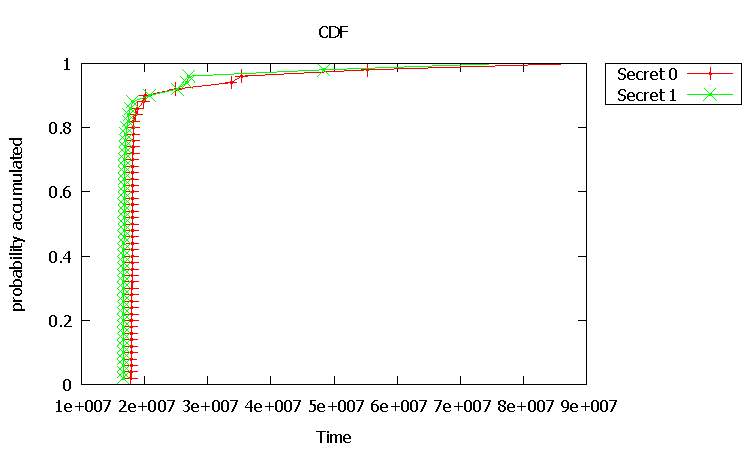
\includegraphics[width=1.0\textwidth]{../::out:::/graphs/CDF.pdf}
	\caption[Results unfiltered: CDF.]{CDF}
  \label{fig:cdf}
	\end{figure}
\newpage

\subsection{Histogram}\label{subsection4}
A \emph{Histogram} shows the distribution of the different data sets.
	\begin{figure}[ht]
	\includegraphics[width=1.0\textwidth]{../::out:::/graphs/histogram.pdf}
	\caption[Results unfiltered: Histogram.]{Histogram}
  \label{fig:histogram}
	\end{figure}
\newpage

\subsection{Secrets in Detail}\label{subsection5}

\subsubsection{Summary}\label{subsubsection1}


\chapter{Results filtered}\label{chapter2}
\section{Statistical Evaluation}\label{section21}
	\newpage
\section{Filtered Scatterplot}\label{section22}
		\begin{figure}[ht]
	\includegraphics[width=1.0\textwidth]{../::out:::/graphs/filtered/scatterplot.pdf}
	\caption[Results filtered: Scatterplot.]{Filtered Scatterplot}
  \label{fig:filteredScatterplot}
	\end{figure}
	\newpage
	
	\section{Filtered Whisker Diagram}\label{section23}
		\begin{figure}[ht]
	\includegraphics[width=1.0\textwidth]{../::out:::/graphs/filtered/whiskerDiagram.pdf}
	\caption[Results filtered: Whisker Diagram.]{Filtered Whisker Diagram}
  \label{fig:filteredWhiskerDiagram}
	\end{figure}
	\newpage
	
	\section{Filtered CDF}\label{section24}
		\begin{figure}[ht]
	\includegraphics[width=1.0\textwidth]{../::out:::/graphs/filtered/cdf.pdf}
	\caption[Results filtered: CDF.]{Filtered CDF}
  \label{fig:filteredCDF}
	\end{figure}
	\newpage
	
	\section{Filtered Histogram}\label{section25}
		\begin{figure}[ht]
	\includegraphics[width=1.0\textwidth]{../::out:::/graphs/filtered/histogram.pdf}
	\caption[Results filtered: Histogram.]{Filtered Histogram}
  \label{fig:filteredHistogram}
	\end{figure}
	\newpage


\chapter{Measurement}\label{chapter3}
\section{Table}\label{section31}
::name:::
\begin{longtable}{|l|l|l|l|l|l|}
\hline
::Spalte1::: & ::Spalte2::: & ::Spalte3::: & ::Spalte4::: & ::Spalte5::: & ::Spalte6::: \\
\hline
\hline
::tableContent:::
\end{longtable}
\newpage

%% Bibliography and other lists
\addtocontents{toc}{\protect\vspace*{\baselineskip}}

%% Appendices
\appendix

\addcontentsline{toc}{chapter}{Appendix}

\pagenumbering{Roman}
\chapter{Scatterplot}
	\begin{figure}[h]
	\rotatebox[origin]{90}{\includegraphics[width=1.0\textwidth]{../::out:::/graphs/scatterplot.pdf}} 	
	\caption[Results unfiltered: Scatterplot.]{Scatterplot}
  \label{appendix:unfiltered:scatterplot}
	\end{figure}
	
\chapter{Whisker Diagram}
	\begin{figure}[h]
	\rotatebox[origin]{90}{\includegraphics[width=1.0\textwidth]{../::out:::/graphs/whiskerDiagram.pdf}} 	
    \caption[Results unfiltered: Whisker Diagram.]{Whisker Diagram}
    \label{appendix:unfiltered:whiskerDiagram}
   	\end{figure}
   	
\chapter{CDF}
	\begin{figure}[h]
	\rotatebox[origin]{90}{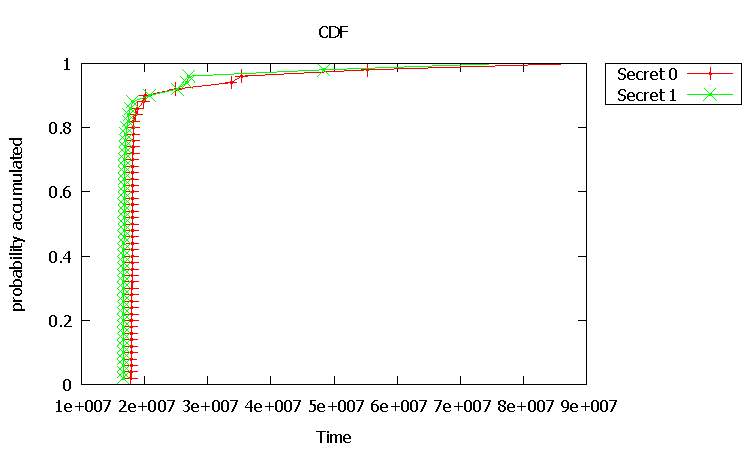
\includegraphics[width=1.0\textwidth]{../::out:::/graphs/CDF.pdf}} 	
    \caption[Results unfiltered: CDF.]{CDF}
    \label{appendix:unfiltered:cdf}
   	\end{figure}
   	
\chapter{Histogram}
	\begin{figure}[h]
	\rotatebox[origin]{90}{\includegraphics[width=1.0\textwidth]{../::out:::/graphs/histogram.pdf}} 	
    \caption[Results unfiltered: Histogram.]{Histogram}
    \label{appendix:unfiltered:histogram}
   	\end{figure}
   	
\chapter{Scatterplot}
	\begin{figure}[h]
	\rotatebox[origin]{90}{\includegraphics[width=1.0\textwidth]{../::out:::/graphs/filtered/scatterplot.pdf}} 	
    \caption[Results filtered: Scatterplot.]{Scatterplot}
    \label{appendix:filtered:scatterplot}
   	\end{figure}
   	
\chapter{Whisker Diagram}
	\begin{figure}[h]
	\rotatebox[origin]{90}{\includegraphics[width=1.0\textwidth]{../::out:::/graphs/filtered/whiskerDiagram.pdf}} 	
    \caption[Results filtered: Whisker Diagram.]{Whisker Diagram}
    \label{appendix:filtered:whiskerDiagram}
   	\end{figure}
   	
\chapter{CDF}
	\begin{figure}[h]
	\rotatebox[origin]{90}{\includegraphics[width=1.0\textwidth]{../::out:::/graphs/filtered/cdf.pdf}} 	
    \caption[Results filtered: CDF.]{CDF}
    \label{appendix:filtered:cdf}
   	\end{figure}
   	
\chapter{Histogram}
	\begin{figure}[h]
	\rotatebox[origin]{90}{\includegraphics[width=1.0\textwidth]{../::out:::/graphs/filtered/histogram.pdf}} 	
    \caption[Results filtered: Histogram.]{Histogram}
    \label{appendix:filtered:histogram}
   	\end{figure}

\end{document}

